%
%  untitled
%
%  Created by Joan T. Matamalas Llodrà on 2011-04-19.
%  Copyright (c) 2011 __MyCompanyName__. All rights reserved.
%
\documentclass[12pt, a4paper]{article}

% Use utf-8 encoding for foreign characters
\usepackage[utf8]{inputenc}

% Setup for fullpage use
\usepackage{fullpage}

% Uncomment some of the following if you use the features
%
% Running Headers and footers
%\usepackage{fancyhdr}

% Multipart figures
\usepackage{subfigure}

% More symbols
%\usepackage{amsmath}
%\usepackage{amssymb}
%\usepackage{latexsym}

% Surround parts of graphics with box
\usepackage{boxedminipage}

% Multirow tables
\usepackage{multirow} 

% Package for including code in the document
\usepackage{listings}

% If you want to generate a  for each chapter (use with book)
%\usepackage{mini}

% This is now the recommended way for checking for PDFLaTeX:
\usepackage{ifpdf}

%\newif\ifpdf
%\ifx\pdfoutput\undefined
%\pdffalse % we are not running PDFLaTeX
%\else
%\pdfoutput=1 % we are running PDFLaTeX
%\pdftrue
%\fi



\ifpdf
\usepackage[pdftex]{graphicx}
\else
\usepackage{graphicx}
\fi
\title{Work 2\\Introduction to Machine Learning}
\author{Marc Oliu \& Joan T. Matamalas}

\date{\today}

\begin{document}

\ifpdf
\DeclareGraphicsExtensions{.pdf, .jpg, .png}
\else
\DeclareGraphicsExtensions{.eps, .jpg}
\fi

\maketitle

\tableofcontents

\listoftables

\newpage

\section{Architecture of the code} % (fold)
\label{sec:architecture_of_the_code}
\paragraph{}The architecture of the code is divided into different function files and a main.m script which contains the main algorithm.\\

First the main script loads all of the datasets from the 10 folds and saves them into a cell matrix, having thus all the combinations of train and test folds loaded into memory to speed up the next step in the execution.\\

Then two nested loops are executed that iterate through a combination of K and R values, where K represents the number of neighbors to be used when apply the KNN algorithms, and R represents the type of distance operator to be used when calculating the distance between elements in the training space with respect to the test element.\\

The R value can take the following values:
\begin{itemize}
	\item 1 = Manhattan distance
	\item 2 = Euclidean distance
	\item 3 = Cubic distance
\end{itemize}
\paragraph{}And the K value, take the value of all the odd numbers in the range from 1 to 13.\\

For each combination of K and R values, the different folds of the dataset will be processed using the CBR algorithm (explained at section 1.5), which will return for each fold the degree of success of the classification process over the test data.\\

When the success degree of the classification for all the folds for a combination of K and R are calculated, the data is used to calculate the mean, the standard deviation and the standard error of means of this success, and these values are printed on screen.\\

After the computation of all combinations of K and R, a graphic representation of the mean accuracy for each combination is plotted. This plot also includes the representation of the confidence interval for each combination. This C.I. is computed with an alpha value of 0.05 using a two tailed Student’s T distribution with nine degrees of freedom.\\

For the second part of the exercise, the values of K and R that gave the best mean accuracy, without taking into account their statistical significance, are automatically selected, and the CBR using this values and different versions of kNN (simple, weighted, selected), giving the mean accuracy standard deviation and the standard error mean for all three algorithms.\\

With this values computed, we perform two different hypothesis tests. The first one two tailed paired t-test, a parametric test. And the second one, Wilcoxon signed-rank test, a non-parametric test.\\

This test are performed by the combinations:
\begin{itemize}
	\item kNN \emph{vs} weightedKNN
	\item kNN \emph{vs} selectedKNN
	\item weightedKNN \emph{vs} selectedKNN
\end{itemize}

\paragraph{}The hypothesis test is as follows:
\begin{itemize}
	\item $H_0: \mu_1 = \mu_2$
	\item $H_1: \mu_1 \neq \mu_2$
\end{itemize}
\paragraph{}The results of that test are shown displaying the relevance of the difference between the used algorithms.

\subsection{The 10-fold parser} % (fold)
\label{sub:the_10_fold_parser}
\paragraph{}The 10-fold parser is divided into two functions. The core one is the \emph{parser\_arff.m} function, which parses a specific file by parsing each data row and transforming the row to a row of integers before adding it to the output matrix.\\

The main difference between this parser and the one implemented in the previous practical work is that now the column representing the classification for each individual is also parsed. To do so, the Attribute line of the file representing the output class column is parsed, and its set of possible classes is saved inside a vector.\\

Then, this vector is used to convert the last parameter of each parsed row to an integer value, which corresponds to the index of the class name inside of the classes vector. This is done so that all rows in all files for the set of files of the same problem have the same value assigned to each class name.\\

When all of the data is parsed, a matrix containing the feature columns and the output class columns is returned by the function, along with a vector that contains the ordered list of output classes.\\

The reason why the classes are converted to an integer value is that, by one side, it's the only way to have both features and output classes inside a matrix, since \emph{Matlab} would create a cell matrix to store mixed fields, and that would make it harder to work with the data. Also, another reason is that the comparison of integer elements is much faster than string elements.\\

The second function of the parser is the one contained inside the \emph{parser\_nfold.m} file, and it's function is to, given a set name and a number of fold, find the test and train files for that set and fold, call the \emph{parser\_arff} function for each file, return the matrixes and parse the output classes glossary (the relation between the class names and their index).

% subsection the_10_fold_parser (end)
\subsection{The kNN implementation} % (fold)
\label{sub:the_knn_implementation}
\paragraph{}The implementation of the kNN algorithm is a really simple one.\\

What is done is to calculate the distances from all of the training set individuals to the test set individual being classified, and then the K nearest neighbors of the training set (those with the shortest distance to the individual) are returned, along with a vector of distances containing the distance to each point.
% subsection the_knn_implementation (end)

\subsection{The weighted kNN implementation} % (fold)
\label{sub:the_weighted_knn_implementation}
\paragraph{}The weighted kNN algorithm we've implemented uses the \emph{relieff} algorithm to calculate the weight for each feature of the data set, and then applies the calculated weight to the distance between the two points for the given dimension by multiplying the distance by the weight.\\

The \emph{relieff} algorithm, for efficiency reasons, is used in the CBR instead of inside the weighted kNN, to prevent the features from being weighted each time a new instance of the train matrix is classified. The weights, as the standardization, are computed at the beginning of the execution of the CBR algorithm, and when a new instance is included into the data base.\\

The weights establishes how important is each feature to determine the similarity between the several instances of the data set.\\

The exact formula to calculate the distance between individuals by taking the weights, \emph{w}, into account is:
\[
	wDistance(x, y) = (\sum_{i=1}^{n}{w_i\cdot|x_i-y_i|^r})^\frac{1}{r}
\]
\paragraph{}Where \emph{x} and \emph{y} are the two individuals for which the distance is calculated, \emph{i} represents the dimension (within \emph{n} features) and \emph{r} is the index of the Minkowski distance being used.\\

The \emph{relieff} algorithm to obtain the weights of the features is an iterative algorithm provided by \emph{Matlab}\footnote{A \emph{filter} to perform feature selection}, which consists on, for each element of the training dataset, calculate the distance to the nearest miss and nearest hit individuals of the set for each feature, and divide this distances by the index of the element currently being checked (1 for the fist, \emph{n} for the last element of the training set). Then, the result for the nearest hit is subtracted from the weight for each feature, while the distance for the nearest miss is added to the weight.\\

This means that the first instance checked will have a high effect on the weight of the features, while subsequent instances will modify in a lesser measure this weight, stabilizing the value over time.\\

The implementation given by \emph{Matlab} for this algorithm returns a value between -1 and 1 for each feature (which is normal, since it’s possible that a certain value has a negative net effect, being the distance to the nearest hit larger than the distance to the nearest miss in most cases), but since we’re interested in using this weight as a factor for the distances, a process of normalization is applied later, leaving the weights between 0 and 1.
% subsection the_weighted_knn_implementation (end)
\subsection{The selected kNN implementation} % (fold)
\label{sub:the_selected_knn_implementation}
\paragraph{}Since the kNN algorithms run for only one test individual, and having to select the features from the original dataset and remove the others for each step would be time-consuming, the selection and extraction of relevant features is done once in the CBR algorithm, and then the normal kNN algorithm is called for each test individual, passing the dataset and test individual with only the selected features.\\

This means there is no specific implementation of the selected kNN.\\

For the feature selection, the same algorithm used to weight the features in the weighted kNN algorithm is used (\emph{relieff}), and then all of the features with a weight lower than the mean of the weights is discarded.
% subsection the_selected_knn_implementation (end)
\subsection{The case-based reasoning algorithm} % (fold)
\label{sub:the_case_based_reasoning_algorithm}
\paragraph{}The case-based reasoning (CBR) algorithm is implemented inside the \emph{cbr.m} function file, and it accepts as parameters the train and test matrixes, the K and R values, and a value indicating which kind of kNN algorithm to accept. This last parameter is defined as follows:
\begin{itemize}
	\item 1: normal kNN
	\item 2: weighted kNN
	\item 3: selected kNN
\end{itemize}
\paragraph{}What this algorithm does is, for each member of the test matrix, find the K nearest neighbors in the train matrix, then count the number of retrieved elements for each class and assign to the test element the most polled class.\\

An important part of the process is standardize the data, this step is make inside the CBR algorithm in order to rise the performance. So when kNN is called the data passed as parameter is standardized.\\

It's possible, though, that there are various classes with the same number of predictors. In that case, what is done is take the distance of the different predictors and keep the class which has its predictors closer to the test individual.\\

The distances used to determine the closest neighbors are the ones returned by the specific kNN algorithm. In the case of the normal and selected kNN, the distance is used (depending on the R value, it can be the Manhattan distance, euclidean or cubic), while in the case of the weighted kNN, those distances are computed using the specific weights of each feature.\\

Since the distances had previously been calculated by the specific kNN algorithm, and the vector of distances returned for the predictors, it's not necessary to recalculate them again.\\

After the class has been selected, it's checked that the prediction is correct, and if it is the counter of  successful predictors is increased. Also, if the prediction is correct and the relative\footnote{Relative considering the maximum entropy for for the different number of classes presents in the set} entropy of the the set of k predictors is higher than a certain value (in our case 0.9), the testing instance is learned. The function that calculated the relative entropy (which is in the range 0 – 1) is defined as follows:
\[
	relativeEntropy = \frac{-\sum_{i=1}^{n}{p(x_i)\cdot log_2(p(x_i))}}{log_2(\# Classes)}
\]
\paragraph{}The algorithm also add to the database the cases not correctly predicted, in order to increase the accuracy when a similar case is tested.\\

Finally, once all of the test individuals have been classified, the number of successes is divided by the number of individuals to get the accuracy, and this value is returned by the function.
% subsection the_case_based_reasoning_algorithm (end)
% section architecture_of_the_code (end)
\newpage
\section{Analysis of the datasets} % (fold)
\label{sec:analysis_of_the_datasets}
\paragraph{}In this chapter we're going to analyze two datasets, first applying the case based reasoning (CBR) algorithm we've implemented to different values of K and R to choose the optimal values, and then using those values to check the performance of the different algorithms we've implemented.

\subsection{Analysis of the \emph{pen-based} dataset} % (fold)
\label{sub:analysis_of_the_pen-based_dataset}
\paragraph{}This dataset consists of 10992 instances defined by 16 descriptors, that describe examples of hand-written characters, and is the dataset we're using as an example of big one. There are bigger datasets to choose from, but because of the time needed to compute the optimal values for K and R, and due to the limitations on computing power, it was unfeasible to select a bigger one (it has to be considered that the time needed to compute a dataset by using 10-fold cross-validation increases quadratically with the number of instances).\\

\begin{figure}[ht!]
	\centering
	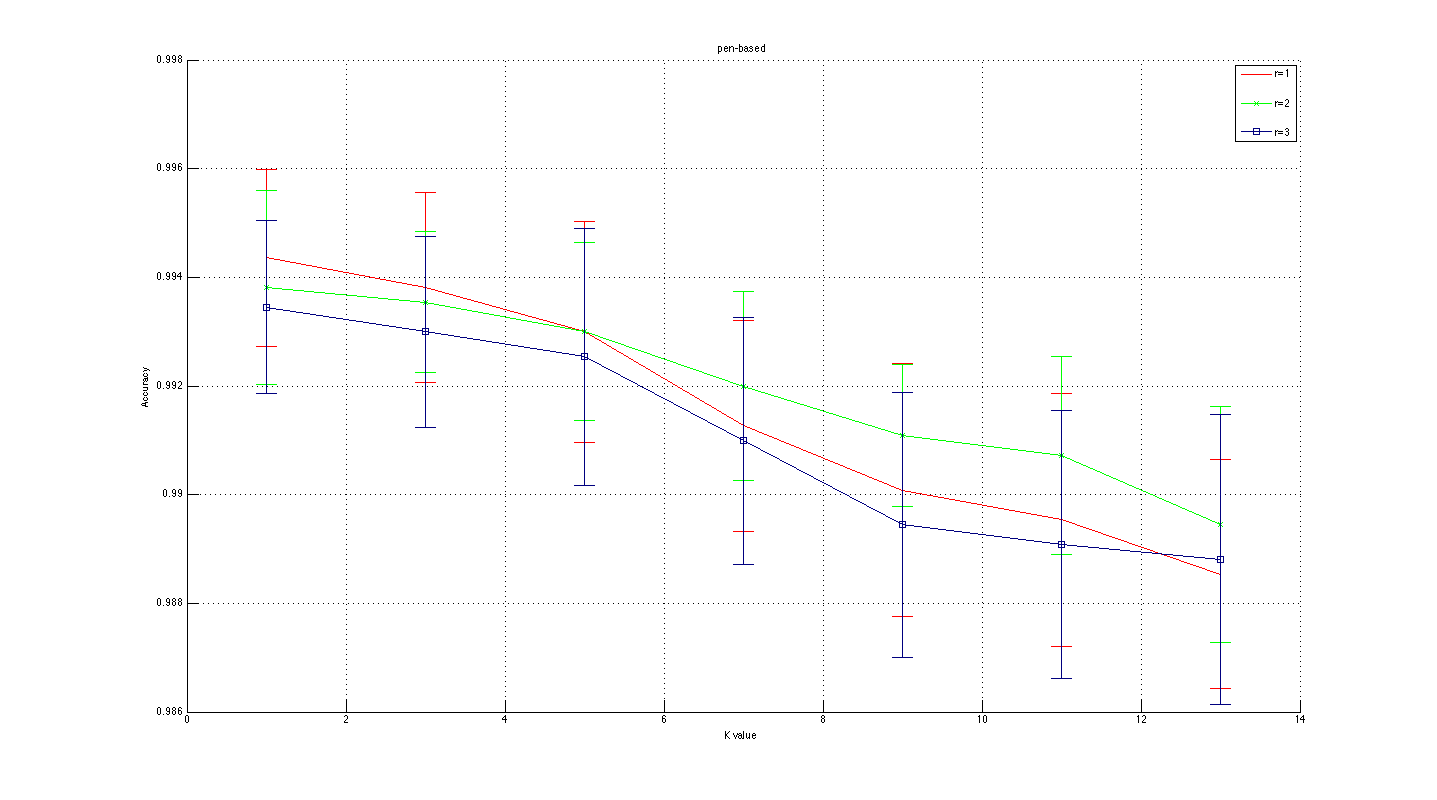
\includegraphics[width=0.99\textwidth]{img/pen-based}
	\caption{Pen-based dataset accuracy evolution}
	\label{fig:pen-based}
\end{figure}
As a first step, we've selected the best values for K and R, by running the CBR algorithm over the ten folds for different combinations of K and R and plotting the solution. The plot we obtained is the following one:\\

It can be seen that the plot represents each R value as a different line in the plot (red for manhattan distance, green for the euclidean distance and blue for the cubic distance). Also, there are two factors to take into account. One is the mean of the ten folds successes. The other one is the confidence interval for this mean, as we have explained in the first section.\\
\begin{table}[ht!]
	\centering
	\small
	\begin{tabular}{|l|c|c|c|}
		\hline
		\textbf&\textbf{kNN}&\textbf{Weighted kNN}&\textbf{Selected kNN}\\\hline
		\textbf{Mean accuracy}& 0.9944 & 0.9944 & 0.9542\\\hline
		\textbf{Accuracy standard deviation} & 0.0019 & 0.0020 & 0.0065\\\hline
		\textbf{Standard Error of Mean} & 0.0007 & 0.0007 & 0.0025\\\hline
	\end{tabular}
	\caption{Statistics values for pen-based dataset}
	\label{tab:statisticsPenBased}
\end{table}

From the results in the above table, it can be seen that the kNN and weighted kNN implementations yield the best results, while the selected kNN implementation lowers the results a little bit.\\

The next step is to analyze these results by applying a paired t-test to contrast the kNN accuracy results with the weighted and selected kNN algorithms. In the section 1, we have already explained the contrast hypothesis parameters.\\

In the first case, for the pair kNN and weighted kNN, the t-test yields the following results:\\
\begin{table}[ht!]
	\centering
	\small
	\begin{tabular}{|lr|}
		\hline
		\textbf{Result} & The $H_0$ cannot be rejected\\
		\textbf{P-value} & 1\\
		\textbf{C.I. for the difference of means} & [-0.0003, 0.0003]\\
		\hline
	\end{tabular}
	\caption{t-test: kNN \emph{vs} weightedKNN (pen-based)}
\end{table}

The results of Wilcoxon test are the following ones:\\
\begin{table}[ht!]
	\centering
	\small
	\begin{tabular}{|lr|}
		\hline
		\textbf{Result} & The $H_0$ cannot be rejected\\
		\textbf{P-value} & 1\\
		\hline
	\end{tabular}
	\caption{Wilcoxon test: kNN \emph{vs} weightedKNN (pen-based)}
\end{table}

In this case, the H0 cannot be rejected, being the means for both cases no show any statistical difference in any of both tests. It can also be seen by looking at the confidence interval, given by the t-test, where the difference of means is centered at zero.\\
\newpage
In the second case, for the pair kNN and selected kNN, the t-test yields the following results:\\
\begin{table}[ht!]
	\centering
	\small
	\begin{tabular}{|lr|}
		\hline
		\textbf{Result} & The $H_0$ is rejected\\
		\textbf{P-value} & 0.0000\\
		\textbf{C.I. for the difference of means} & [0.0351, 0.0451]\\
		\hline
	\end{tabular}
	\caption{t-test: kNN \emph{vs} selected kNN (pen-based)}
\end{table}

And the Wilcoxon test:\\
\begin{table}[ht!]
	\centering
	\small
	\begin{tabular}{|lr|}
		\hline
		\textbf{Result} & The $H_0$ is rejected\\
		\textbf{P-value} & 0.0020\\
		\hline
	\end{tabular}
	\caption{Wilcoxon test: kNN \emph{vs} selected KNN (pen-based)}
\end{table}

Finally the results for the t-test and Wilcoxon test for weighted kNN and selected kNN:\\
\begin{table}[ht!]
	\centering
	\small
	\begin{tabular}{|lr|}
		\hline
		\textbf{Result} & The $H_0$ is rejected\\
		\textbf{P-value} & 0.0000\\
		\textbf{C.I. for the difference of means} & [0.0350, 0.0452]\\
		\hline
	\end{tabular}
	\caption{t-test: weighted kNN \emph{vs} selected kNN (pen-based)}
\end{table}
\begin{table}[ht!]
	\centering
	\small
	\begin{tabular}{|lr|}
		\hline
		\textbf{Result} & The $H_0$ is rejected\\
		\textbf{P-value} & 0.0020\\
		\hline
	\end{tabular}
	\caption{Wilcoxon test: weighted kNN \emph{vs} selected KNN (pen-based)}
\end{table}

In this case, the $H_1$ hypotheses is true with a significance level of alpha 0.05, that is, both accuracies distributions have a different mean, in both tests.\\

As a conclusion, based in the statistical results of the t-test and Wilcoxon test, we can say that the kNN and weighted kNN algorithms have the same prediction power, while the selected kNN has a lower prediction power than the other two.\\

Now we can take a look at the variables that were discarded by the selected kNN algorithm:
\begin{itemize}
	\item \textbf{Attribute a1}: Selected
	\item \textbf{Attribute a2}: Discarded
	\item \textbf{Attribute a3}: Discarded
	\item \textbf{Attribute a4}: Discarded
	\item \textbf{Attribute a5}: Selected
	\item \textbf{Attribute a6}: Discarded
	\item \textbf{Attribute a7}: Selected
	\item \textbf{Attribute a8}: Selected
	\item \textbf{Attribute a9}: Discarded
	\item \textbf{Attribute a10}: Selected
	\item \textbf{Attribute a11}: Selected
	\item \textbf{Attribute a12}: Discarded
	\item \textbf{Attribute a13}: Discarded
	\item \textbf{Attribute a14}: Selected
	\item \textbf{Attribute a15}: Selected
	\item \textbf{Attribute a16}: Selected		 
\end{itemize}
\paragraph{}As it can be seen, 7 of the 16 features, almost half of them, have been discarded during the feature selection process. If we consider that the predicting power went down from 99.44\% to 95.42\%. As it can be seen, 7 of the 16 features, almost half of them, have been discarded during the feature selection process. If we consider that the predicting power went down from 99.44\% to 95.42\%. This difference can be critical or not depending on the context where has to be applied. For instance, the goal of the classification is to recognize hand-written characters, if this characters have to be used in a hand-written formula to \LaTeX~application, this loss of accuracy seems acceptable. However, if the application is used to read a paycheck amount, this loss of accuracy seems critical. So, depending on the circumstances, the loss of accuracy seems acceptable in exchange of a increase in the performance of the algorithm and a simplification of the model. It would also be useful to find out which are the relevant variables of the problem, and thus to know better the underlying information of the classification problem.
% subsection analysis_of_the_pen-based_dataset (end)

\subsection{Analysis of the \emph{breast-w} dataset} % (fold)
\label{sub:analysis_of_the_breast-w_dataset}
\paragraph{}This data set contains 699 instances defined by nine descriptors, that classify a determined test cancer has \emph{benign} or \emph{malignant}. So we will consider the accuracy of the system a critical aspect.\\

First, we need to execute the CBR with 10 different test sets (10 fold cross-validation) as we did in the previous analysis. The next plot shows the evolution of accuracy, for several values of K and R.\\

As we have commented in the first section of this paper, for each value of K and R we plot the mean accuracy of the results of the cross-validation and the confidence interval for this values.\\

As we can see, all the accuracy values remain in a 2\% range. And, as in the previous dataset, there is overlapping between some confidence intervals, which makes it hard to decide which value of K and R are the better ones. Applying the same criterion that in the case of the pen-based dataset, we’ve selected K=3 and R = 1.\\

\begin{figure}[ht!]
	\centering
	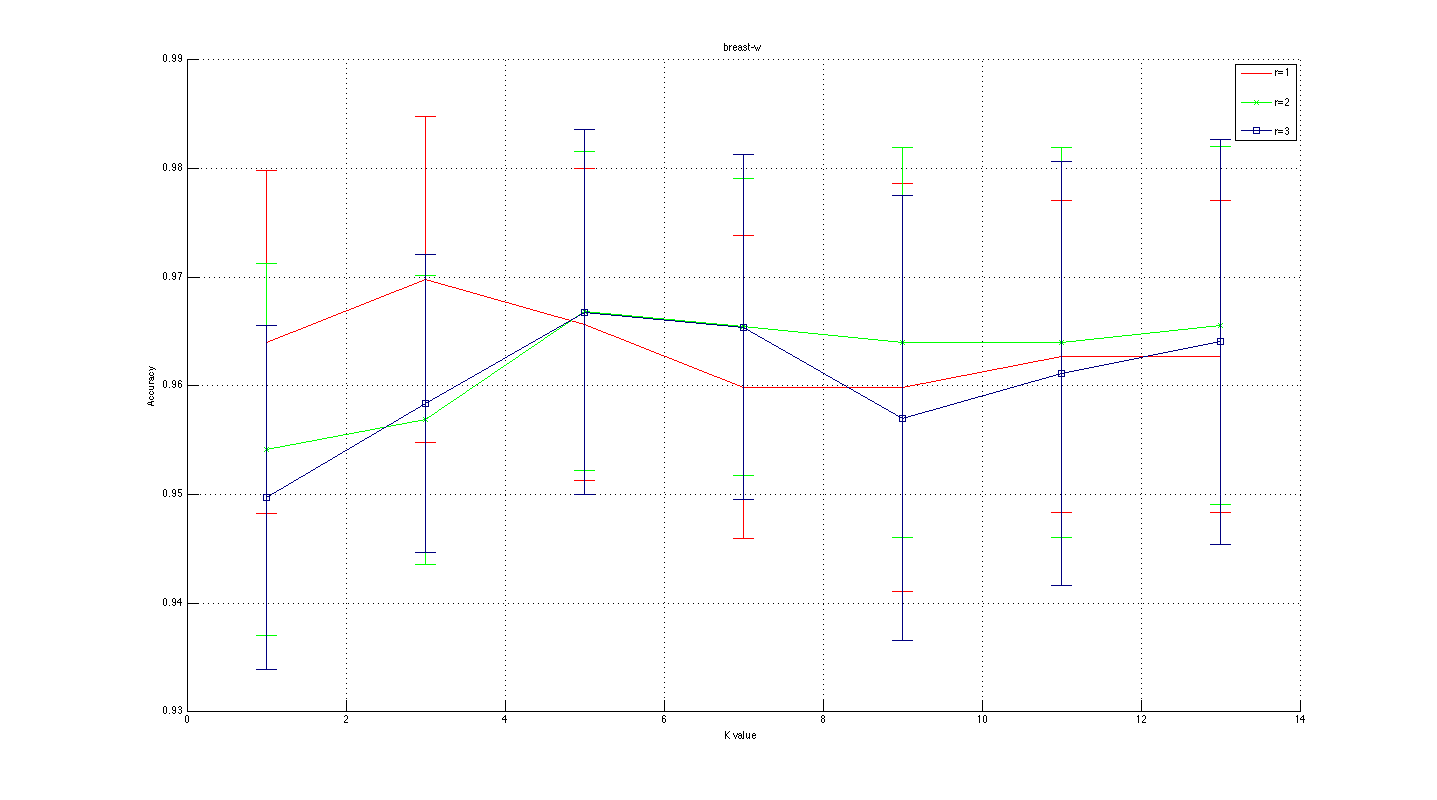
\includegraphics[width=0.99\textwidth]{img/breast-w}
	\caption{Breast-w dataset accuracy evolution}
	\label{fig:breast-w}
\end{figure}

The next step is run the CBR algorithm with weightedKNN and selectedKNN with these values of K and R. In the following table we’ll show this results:\\
\begin{table}[ht!]
	\centering
	\small
	\begin{tabular}{|l|c|c|c|}
		\hline
		\textbf&\textbf{kNN}&\textbf{Weighted kNN}&\textbf{Selected kNN}\\\hline
		\textbf{Mean accuracy}& 0.9698 & 0.9684 & 0.9469\\\hline
		\textbf{Accuracy standard deviation} & 0.0175 & 0.0166 & 0.0275\\\hline
		\textbf{Standard Error of Mean} & 0.0066 & 0.0063 & 0.0104\\\hline
	\end{tabular}
	\caption{Statistics values for breast-w dataset}
	\label{tab:statisticsBreastW}
\end{table}

Now, with the accuracy values collected for each specific algorithm we can compare statistically this results with a two tailed paired t-test.\\

Let’s begin with the comparative between the results of CBR using the kNN versus the one that uses the weightedKNN:\\
\begin{table}[ht!]
	\centering
	\small
	\begin{tabular}{|lr|}
		\hline
		\textbf{Result} & The $H_0$ cannot be rejected\\
		\textbf{P-value} & 0.5983\\
		\textbf{C.I. for the difference of means} & [-0.0044, 0.0072]\\
		\hline
	\end{tabular}
	\caption{t-test: kNN \emph{vs} weighted kNN (breast-w)}
\end{table}
\begin{table}[ht!]
	\centering
	\small
	\begin{tabular}{|lr|}
		\hline
		\textbf{Result} & The $H_0$ cannot be rejected\\
		\textbf{P-value} & 1.0000\\
		\hline
	\end{tabular}
	\caption{Wilcoxon test: kNN \emph{vs} weighted KNN (breast-w)}
\end{table}

That result shows no statistical difference among the accuracy obtained classifying using the kNN and the weightedKNN.\\

Now, let’s see the comparative between the accuracy of the CBR using the kNN vs the version that uses the selectedKNN.\\
\begin{table}[ht!]
	\centering
	\small
	\begin{tabular}{|lr|}
		\hline
		\textbf{Result} & The $H_0$ is rejected\\
		\textbf{P-value} & 0.0047\\
		\textbf{C.I. for the difference of means} & [0.0090, 0.0367]\\
		\hline
	\end{tabular}
	\caption{t-test: kNN \emph{vs} selected kNN (breast-w)}
\end{table}
\begin{table}[ht!]
	\centering
	\small
	\begin{tabular}{|lr|}
		\hline
		\textbf{Result} & The $H_0$ is rejected\\
		\textbf{P-value} & 0.0156\\
		\hline
	\end{tabular}
	\caption{Wilcoxon test: kNN \emph{vs} selected KNN (breast-w)}
\end{table}

Finally, the comparative between weighted and selected kNN:
\begin{table}[ht!]
	\centering
	\small
	\begin{tabular}{|lr|}
		\hline
		\textbf{Result} & The $H_0$ is rejected\\
		\textbf{P-value} & 0.0188\\
		\textbf{C.I. for the difference of means} & [0.0045, 0.0384]\\
		\hline
	\end{tabular}
	\caption{t-test: weighted kNN \emph{vs} selected kNN (breast-w)}
\end{table}
\begin{table}[ht!]
	\centering
	\small
	\begin{tabular}{|lr|}
		\hline
		\textbf{Result} & The $H_0$ is rejected\\
		\textbf{P-value} & 0.0312\\
		\hline
	\end{tabular}
	\caption{Wilcoxon test: weighted kNN \emph{vs} selected KNN (breast-w)}
\end{table}

The accuracy of the CBR using the kNN and weightedKNN algorithms to classify the instances of the test set are statistically better, with a 95\% of confidence, than the accuracy obtained using the kNN version that discriminates between features. That seems an important difference considering the context where this classifier can be potentially applied. So we consider recommendable the use of the CBR that uses kNN or weighted kNN instead the one that uses a selected set of features.\\

The weights, as we commented earlier, are computed for the train set when the CBR starts its execution, and recomputed when an additional instance is \emph{learned} from the test set. This fact can alter the features used in selected kNN, because the process just selects the features that lie beyond the weights mean, and this value may change as the weights are changed.\\

However, two features of the set have always been selected in all the folds:
\begin{itemize}
	\item Clump\_Thickness
	\item Bare\_Nuclei
\end{itemize}
\paragraph{}In some fold execution and in some periods of time, the next two variables have also been selected:
\begin{itemize}
	\item Cell\_Size\_Uniformity
	\item Cell\_Shape\_Uniformity
\end{itemize}
\paragraph{}Those factors could be interesting to analyze in order to determine the principal factors of the analysis but, as we’ve mentioned, taking into account the different accuracy values, we strongly recommend the use of the CBR using the standard kNN for classification tasks, given the critical context where the classifier could be applied.
% subsection analysis_of_the_breast-w_dataset (end)
% section analysis_of_the_datasets (end)
\bibliographystyle{plain}
\bibliography{}
\end{document}
